The work focuses on properties enjoyed by the lattice of noncrossing partitions $\text{NC}(n)$, but not by the lattice of all partitions $\Pi(n)$, namely self-duality (which implies rank symmetry) and symmetric chain decomposition. Based on these results, several equalities are derived.

\section{Introduction and Notations}

A \textit{noncrossing partition} $\pi$ of $[n]=\{1,\ldots,n\}$ is a partition of $[n]$ into blocks, such that whenever $1\le a<b<c<d\le n$ and $a$ and $c$ are in the same block (later denoted as $a\sim_{\pi} c$) and $b$ and $d$ are in the same block, then $a,b,c,d$ are in the same block. That means when drawing the numbers as points in a circle in clockwise or counter-clockwise order and connecting each pair in the same block with a chord, no two chords from distinct blocks intersect.. Henceforth, $a\sim_\pi b$ if and only if there is a chord $ab$ in the cyclic representation of $\pi$ (or briefly, in $\pi$). For example, $\{\{1,3,8\},\{2\},\{4\}, \{5,7\},\{6\}\}$, from now on written briefly as $138|2|4|57|6$, is a noncrossing partition of $[8]$, while $138|24|57|6$ is not, as shown in Figures \ref{fig:1a} and \ref{fig:1b}, respectively.

\begin{figure}[h]
  \centering
  \begin{subfigure}{0.32\textwidth}
    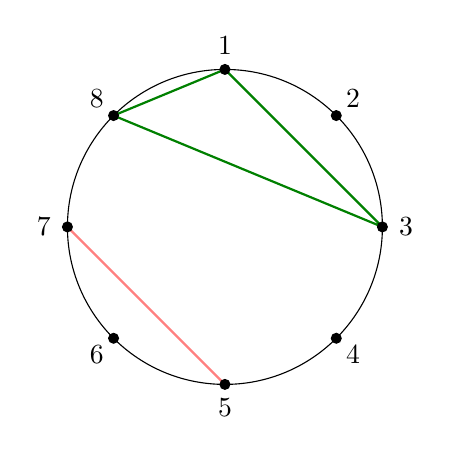
\begin{tikzpicture}
      \draw (0,0) circle (2);

      \draw[thick, color=red!50] (135-5*45:2) -- (135-7*45:2);

      \draw[thick, color=green!50!black] (135-1*45:2) -- (135-3*45:2) -- (135-8*45:2) -- cycle;
      \foreach \n in {1,...,8} {
          \fill (135-\n*45:2) circle (2pt);
          \node at (135-\n*45:2.3) {$\n$};
        }
    \end{tikzpicture}
    \caption{}
    \label{fig:1a}
  \end{subfigure}
  \begin{subfigure}{0.32\textwidth}
    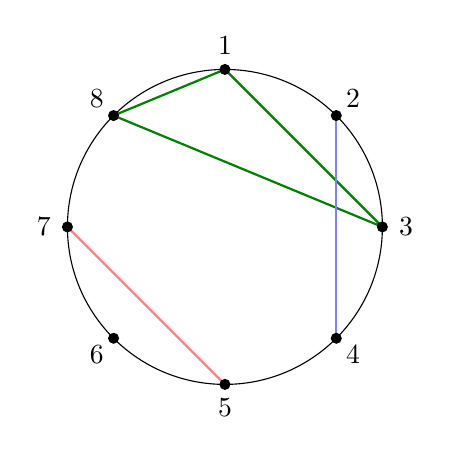
\begin{tikzpicture}
      \draw (0,0) circle (2);

      \draw[thick, color=green!50!black] (135-1*45:2) -- (135-3*45:2) -- (135-8*45:2) -- cycle;
      \draw[thick, color=blue!50] (135-2*45:2) -- (135-4*45:2);

      \draw[thick, color=red!50] (135-5*45:2) -- (135-7*45:2);

      \foreach \n in {1,...,8} {
          \fill (135-\n*45:2) circle (2pt);
          \node at (135-\n*45:2.3) {$\n$};
        }
    \end{tikzpicture}
    \caption{}
    \label{fig:1b}
  \end{subfigure}
  \begin{subfigure}{0.32\textwidth}
    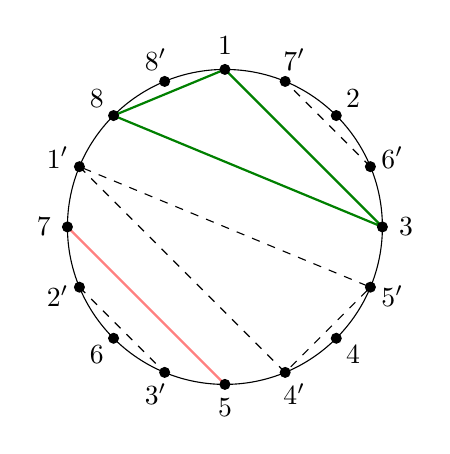
\begin{tikzpicture}
      \draw (0,0) circle (2);

      \draw[thick, color=red!50] (135-5*45:2) -- (135-7*45:2);

      \draw[thick, color=green!50!black] (135-1*45:2) -- (135-3*45:2) -- (135-8*45:2) -- cycle;
      \foreach \n in {1,...,8} {
          \fill (135-\n*45:2) circle (2pt);
          \node at (135-\n*45:2.3) {$\n$};
          \fill (112.5+\n*45:2) circle (2pt);
          \node (\n_prime) at (112.5+\n*45:2.3) {$\n'$};
        }

      \draw[dashed] (112.5+1*45:2) -- (112.5+4*45:2) -- (112.5+5*45:2)-- (112.5+1*45:2);
      \draw[dashed] (112.5+6*45:2) -- (112.5+7*45:2);
      \draw[dashed] (112.5+2*45:2) -- (112.5+3*45:2);
    \end{tikzpicture}
    \caption{}
    \label{fig:1c}
  \end{subfigure}
  \caption{}
  \label{fig:1}
\end{figure}

We also consider the linear representation, where the numbers are drawn on a line and a semicircle is drawn for each consecutive pair in the same block. For example, the linear representation of $138|2|4|57|6$ is shown in Figure \ref{fig:2}. This allows us to speak of \textit{nested blocks}. For example, in the same figure, the block $57$ is nested in the block $138$.

\begin{figure}[ht]
  \centering
  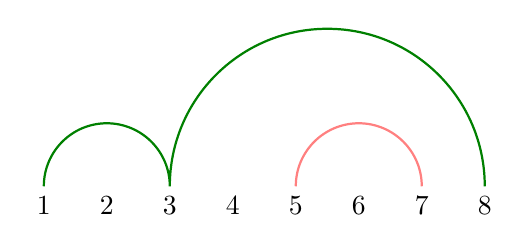
\begin{tikzpicture}[scale=0.8]
    \foreach \n in {1,...,8} {
        \node at (\n,-0.3) {$\n$};
      }

    \draw[thick, color=green!50!black] (1,0) arc (180:0:1) (3,0) arc (180:0:2.5) (8,0);
    \draw[thick, color=red!50] (5,0) arc (180:0:1);
  \end{tikzpicture}
  \caption{}
  \label{fig:2}
\end{figure}

The number of noncrossing partitions of $[n]$ is the $n$-th Catalan number $C_n$. The number of noncrossing partitions of $[n]$ having $i$ blocks is $W(n,i)=\frac{1}{n}\binom{n}{i}\binom{n}{i-1}$.

The \textit{refinement order} on $\Pi(n)$, denoted by $\leq$,  is defined by $\pi \leq \pi'$ if every block of $\pi$ is contained in a block of $\pi'$. For example, $138|2|4|57|6 \leq1382|567$. We also denote by $\pi\lessdot \pi'$ the fact that $\pi'$ covers $\pi$ i.e. $\pi \leq \pi'$ and there is no partition $\pi''$ such that $\pi < \pi'' < \pi'$. That means $\pi'$ is obtained from $\pi$ by merging two blocks of $\pi$. The \textit{rank} of a partition $\pi$ is defined as $\text{rk}(\pi) = n - \text{bk}(\pi)$, where $\text{bk}(\pi)$ is the number of blocks of $\pi$.

\section{Properties}
\begin{theorem}
  For each $n\ge 1$, the lattice $\text{NC}(n)$ is self-dual. That is, there is an order-reversing bijection $\alpha: \text{NC}(n) \to \text{NC}(n)$ such that $\pi \leq \pi'$ iff $\alpha(\pi') \leq \alpha(\pi)$ for any $\pi, \pi' \in \text{NC}(n)$.
\end{theorem}

\begin{proof}
  Define $\alpha$ such that $i'<j'$ and $i'\sim_{\alpha(\pi)}j'$ iff there is no $i < j$ and $i\sim_{\pi}j$ with either $i' < n+1-j \le j' < n+1-i$ or $n+1-j \le i' < n+1-i \le j'$. In the cyclic representation above, that means
  \begin{enumerate}
    \item Replace each $i$ by $n+1-i$ for all $i\in [n]$.
    \item Draw a point $i'$ (it has value $i$, but distinguished from $i$) between $i$ and $i+1$, with convention that $n+1$ is identified with $1$.
    \item Draw a chord between $i'$ and $j'$ iff it crosses no initial chord.
    \item Revert the first step, i.e. replace each $i$ by $n+1-i$ for all $i\in [n]$.
  \end{enumerate}

  Let us show that $\sim_{\alpha(\pi)}$ is transitive. Let $i'<j'$, $i'\sim_{\alpha(\pi)}k'$ and $j'\sim_{\alpha(\pi)}k'$. Suppose that $i'\not\sim_{\alpha(\pi)}j'$. Consider the case that there is $i<j$ with $i' < n+1-j \le j' < n+1-i$ (the other case is similar), or equivalently, $i' \le n-j < j' \le n-i$. Consider the cases
  $$k'<i'; \quad i'<k'\le n-j; \quad n-j < k' < j'; \quad j' < k' \le n-i; \quad n-i < k',$$
  we arrive at a contradiction in all cases to either $i'\sim_{\alpha(\pi)}j'$ or $j'\sim_{\alpha(\pi)}k'$. Therefore, the new chords correspond to the unique maximal non-crossing partition on $\{1', 2', \dots, n'\}$ whose chords do not cross the initial chords of $\pi$ (an example of $\alpha(138|2|4|57|6)$ is shown in Figure \ref{fig:1c}). Hence, $\alpha$ is well-defined. By definition of $\alpha$, any chord of $\pi$ does not cross any chord of $\alpha(\pi)$. Hence two statements $i<j \wedge i\sim_{\pi}j$ and $i<j \wedge i\sim_{\alpha^2(\pi)}j$ are both equivalent to
  $$\exists i',j': i'<j'\wedge  i'\sim_{\alpha(\pi)}j'\wedge (i' \le n-j < j' \le n-i \vee i' \le n-j < j' \le n-i)$$

  Therefore $\alpha^2 = \text{id}$ i.e. $\alpha$ is an involution, thus a bijection. Now let $\pi\le \pi'$. Then $\alpha(\pi')$ does not cross $\pi'$, hence does not cross $\pi$, while $\alpha(\pi)$ is the maximal that does not cross $\pi$. Therefore, $\alpha(\pi') \le \alpha(\pi)$. Thus, $\alpha$ is an order-reversing bijection, and $\text{NC}(n)$ is self-dual.
\end{proof}

\begin{theorem}
  For each $n\ge 1$, the lattice $\text{NC}(n)$ is rank-symmetric. That is, the number of noncrossing partitions of rank $k$ is equal to the number of noncrossing partitions of rank $n-1-k$ for any $0\le k \le n-1$.
\end{theorem}

\begin{proof}
  Let $\alpha$ be as defined. Let $\pi\lessdot \pi'$, then $\alpha(\pi')\lessdot \alpha(\pi)$.
  Hence $\text{bk}(\pi') = \text{bk}(\pi)+1$ and $\text{bk}(\alpha(\pi')) = \text{bk}(\alpha(\pi))-1$. Therefore, $\text{bk}(\pi') + \text{bk}(\alpha(\pi')) = \text{bk}(\pi) + \text{bk}(\alpha(\pi)).$

  Now regard $\text{NC}(n)$ as a undirected graph. Since $12\ldots n \le \pi$ for any $\pi$, the graph is connected and the previous equality holds for any $\pi$ and $\pi'$. Since $\text{bk}(12\ldots n) = 1$, $\alpha(12\ldots n) = 1|2|\ldots|n$ and $\text{bk}(1|2|\ldots|n) = n$, we have $\text{bk}(\pi) + \text{bk}(\alpha(\pi)) = n+1$ for any $\pi$. Therefore, $\text{rk}(\pi) + \text{rk}(\alpha(\pi)) = n-1$. Hence, the number of noncrossing partitions of rank $k$ is equal to the number of noncrossing partitions of rank $n-1-k$.
\end{proof}

Recall that a symmetric chain decomposition (SCD) of a graded poset $P$ is a partition of $P$ into chains, such that each chain contains elements of ranks $k, k+1, \dots, n-k$ for some $k$.

\begin{theorem}
  For each $n\ge 1$, the lattice $\text{NC}(n)$ admits a symmetric chain decomposition.
\end{theorem}

We outline the nonconstructive proof and focus on the constructive proof for later use.

\begin{proof}[Nonconstructive proof]
  Define $R_i$ to be the set of noncrossing partitions such that the least element in the block containing $1$ is $i$. We have $R_1\cong \text{NC}(n-1)$ (seeing $1$ as empty) and $R_2\cong \text{NC}(n-1)$ (seeing $1$ and $2$ as a single point), hence $R_1\cup R_2\cong \text{NC}(n-1)\times \{0 < 1\}$. Also, $R_i\cong \text{NC}(i-2)\times \text{NC}(n-i+1)$ (identifying $1$ with $i$, then split to two two independent circles $\left\{2,\ldots,i-1\right\}$ and $\left\{i,\ldots,n\right\}$). Using the fact that the product of two posets with SCDs also admits an SCD and checking the base cases, we conclude the result.
\end{proof}

\begin{proof}[Constructive proof]
  We assign to each $\pi\in\text{NC}(n)$ a word $w(\pi) = w_1\ldots w_{n-1}$ over the alphabet $\{b,e,\ell,r\}$ as follows
  $$w_i = \begin{cases}
      b,    & \text{if $i\not\sim_\pi i+1$ and $i$ is \textit{not} the largest element in its block} \\
      e,    & \text{if $i\not\sim_\pi 1$ and $i$ is \textit{not} the smallest element in its block}  \\
      \ell, & \text{if $i\not\sim_\pi i+1$, $i$ is the largest element in its block}                 \\
            & \text{\,\,\,\,and $i+1$ is the smallest element in its block}                          \\
      r,    & \text{if $i\sim_\pi i+1$}
    \end{cases}.$$
  The letter $b$ means there is a nested block of the one containing $i$ that begins at $i+1$. The letter $e$ means there is a nested block of the one containing $i$ that ends at $i$. The letter $\ell$ means new non-nested blocks begins at $i+1$.  The letter $r$ means the block containing $i$ continues at $i+1$.
  Let $B=\{i : w_i = b\}$ (respectively $E$, $L$, $R$).

  \begin{observation}
    \label{obs:b=e}
    We have $|B|+|E|+|L|+|R|=n-1$. Moreover, $1+|B|+|L|$ counts the minimums in the blocks, while $1+|B|+|E|$ counts the maximums. Hence $\text{bk}(\pi) = 1+|B|+|L|=1+|B|+|E|$ and $|B| = |E|$.
  \end{observation}

  \begin{observation}
    Regarding each $b$ in $w(\pi)$ as an opening parenthesis and each $e$ as a closing parenthesis, we have a \textit{complete parenthesization}. Indeed, if $w_i=b$, then there is a block containing $i$ and has elements larger than $i$. Let $j$ be the smallest such element, then $w_{j-1}=e$ and closes the parenthesis opened by $w_i$. Since each pair of parentheses corresponds to two successive elements in the same block, the parenthesization is complete.
  \end{observation}

  \begin{observation}
    \label{obs:boolean}
    Now we see that reading a letter $b$ is going one deeper nested level, while reading a letter $e$ is going one shallower nested level; reading a letter $\ell$ is starting a new block in the same nested level, while reading a letter $r$ is continuing the current block. If we fix the positions of $b$ and $e$, then every choice of $\ell$ and $r$ in the remaining positions corresponds to a valid noncrossing partition. Therefore, the noncrossing partitions with the same $B$ and $E$ form a Boolean lattice isomorphic to $B_{n-1-2|B|}$, and these Boolean lattices are disjoint. Moreover, the correspondence $\pi\mapsto w(\pi)$ induces a bijection between the set of noncrossing partitions and a set of length-$(n-1)$ words in $\{b,e,\ell,r\}^*$ with the same number of $b$'s and $e$'s.
  \end{observation}

  Now also regard the letters $\ell$ and $r$ as opening and closing parentheses. Let $\mathit{ML}$ and $\mathit{MR}$ be the sets of positions of \textit{matched} $\ell$ and $r$. We call $c=(B, E, \mathit{ML},\mathit{MR})$ the \textit{core} of $\pi$. Once we fix that tuple, the minimal corresponding partition is when all the remaining letters are $\ell$ (deciding to exit a block as early as possible). Form a sequence of partition by replacing these $L-\mathit{ML}$ letters $\ell$'s by $r$'s from left to right. We get a saturated chain. Using Observation  \ref{obs:b=e}, the number of blocks in the minimal partition is $n-|E|-|\mathit{MR}|$, while the number of blocks in the maximal partition is $1+|B|+|\mathit{ML}|$. Since $|E| = |B|$ and $|\mathit{MR}| = |\mathit{ML}|$, the chain is symmetric.
\end{proof}



\section{Equalities}
\begin{corollary}[Touchard's identity]
  For every $n\ge 1$, $\sum\limits_{k\ge 0} \binom{n-1}{2k} C_k2^{n-2k-1} = C_n$.
\end{corollary}
\begin{proof}
  We show that the left-hand side counts the number of noncrossing partitions of $[n]$. We count the number of noncrossing partitions with $|B|=|E|=k$. There are $\binom{n-1}{2k}$ ways to choose the positions of $b$'s and $e$'s, $C_k$ ways to match them, and $2^{n-2k-1}$ ways to choose $\ell$ or $r$ for the remaining positions. Summing over $k$ gives the result.
\end{proof}

\begin{corollary}
  For every $n\ge 1$ and $i\in[n]$, $\sum\limits_{k\ge 0} \binom{n-1}{2k} \binom{n-2k-1}{n-k-i}C_k = W(n,i)$.
\end{corollary}

\begin{proof}
  The right-hand side is a known result of the number $W(n,i)$ of partitions having $i$-blocks. We count them in another way, again, for each $k$ such that $|B|=|E|=k$. Using Observation   \ref{obs:b=e}, $i = 1+|B| + |L| = n-|B|-|R|$ or $|R|=n-k-i$. There are $\binom{n-1}{2k}C_k$ ways to choose and match $b$'s and $e$'s and $\binom{n-2k-1}{n-k-i}$ ways to choose $R$. Summing over $k$ gives the result.
\end{proof}

% \begin{corollary}
%   For every $n\ge 1$ and $(n+1)/2\le i\le n$,
%   $$\sum\limits_{k\ge 0} \binom{n-1}{2k} C_k \left[\binom{n-2k-1}{i-k-1}-\binom{n-2k-1}{i-k}\right] = \frac{\binom{n+1}{i}\binom{n-1}{i-1}}{\binom{i+1}{2}}.$$
% \end{corollary}

% \begin{proof}
%   The right-hand side is equal to $W(n,i)-W(n,i+1)$. Consider an SCD of $\text{NC}(n)$, that is, every partition belongs to exactly one symmetric chain. Then $W(n,i)-W(n,i+1)$ counts the number of chains that starts from an $i$-block partitions. Again, we count for each $k$ with $|B|=|E|=k$.
% \end{proof}

\begin{proposition}
  Let $\overline{\text{NC}}(n)$ be the set of noncrossing partitions of $[n]$ with no consecutive elements in the same block and $\text{NC}_2(n)$ be the set of noncrossing partitions of $[n]$ whose blocks have size at most 2. Then $|\overline{\text{NC}}(n)| = |\text{NC}_2(n)|$.
\end{proposition}

\begin{proof}
  Consider the SDC in the constructive proof. Recall Observation \ref{obs:boolean} that the set of partitions with a fixed $(B,E)$ is a boolean lattice. Since the $b$'s and $e$'s are matched, each boolean lattice corresponds bijectively to a partition in $\text{NC}_2(n-1)$, by seeing each pair of matched $b$ and $e$ as a block of size 2 and each remaining position in $[n-1]$ as a block of size 1. On the other hand, we count the boolean lattices by their minimum elements i.e. elements having $R=\varnothing$. Equivalently, $i\not\sim_\pi i+1$ for every $i\in[n-1]$. Hence, each boolean lattice corresponds bijectively to a partition in $\overline{\text{NC}}(n)$. Thus, $|\overline{\text{NC}}(n)| = |\text{NC}_2(n-1)|$.

  A direct bijection can also be defined as follows. For each $\pi\in \overline{\text{NC}}(n)$, write the word representation of $\pi$, then let each matched pair of $b$ and $e$ correspond to a block of size 2, and each remaining letter correspond to a block of size 1. This gives a partition $\pi'$ in $\text{NC}_2(n)$. Conversely, for each $\pi'\in \text{NC}_2(n)$, write the word $w$ with $w_i = b$ and $w_j = e$ for each block of size 2 with minimum $i$ and maximum $j$, and $w_k = \ell$ for each remaining position. This corresponds to a partition $\pi$ in $\overline{\text{NC}}(n)$.
\end{proof}

We also have a recurrence relation for $|\overline{\text{NC}}(n)|$, based on the smallest element $k\in [3,n]$ in the block containing $1$, by identifying $1$ and $k$ and splitting the circle into two independent circles $[1,k-1]$ and $[k,n]$. We have, for each $n\ge 2$,
$$|\overline{\text{NC}}(n)| = \sum_{i=0}^{n-2} |\overline{\text{NC}}(i)| \cdot |\overline{\text{NC}}(n-i-1)|.$$
Note that $\overline{\text{NC}}(0) = \overline{\text{NC}}(1) = 1$. Let $f(x) = \sum_{n=0}^{\infty} |\overline{\text{NC}}(n)|x^n$ be the generating function of $|\overline{\text{NC}}(n)|$. Let $a_n=|\overline{\text{NC}}(n)|$, we have
\begin{align*}
  f(x) & = a_0 + a_1 x  + \sum_{n=2}^{\infty} \sum_{i=0}^{n-2} a_i a_{n-i-1} x^n = 1 + x + x \sum_{n=1}^{\infty} \left[ \left( \sum_{i=0}^{n} a_i a_{n-i} \right) - a_n \right] x^n \\
       & = 1 + x + x f(x)^2 - x f(x).
\end{align*}
Thus,
$$f(x) = \frac{1+x-\sqrt{1-2x-3x^2}}{2x}.$$
